%%%%%%%%%%%%%%%%%%%%%%%%%%%%%%%%%%%%%%%%%%%%%%%%%%
%
%  New template code for TAMU Theses and Dissertations starting Fall 2012.  
%  For more info about this template or the 
%  TAMU LaTeX User's Group, see http://www.howdy.me/.
%
%  Author: Wendy Lynn Turner 
%	 Version 1.0 
%  Last updated 8/5/2012
%
%%%%%%%%%%%%%%%%%%%%%%%%%%%%%%%%%%%%%%%%%%%%%%%%%%%
%%%%%%%%%%%%%%%%%%%%%%%%%%%%%%%%%%%%%%%%%%%%%%%%%%%%%%%%%%%%%%%%%%%%%%
%%                           SECTION IV
%%%%%%%%%%%%%%%%%%%%%%%%%%%%%%%%%%%%%%%%%%%%%%%%%%%%%%%%%%%%%%%%%%%%%

\chapter{\uppercase{Design}}

The primary goal of this thesis is to implement an object detection and tracking system using one of the most well-known visual tracking algorithms and machine learning frameworks from the computer vision field: TensorFlow, YOLO, TLD, and OpenCV. We will make some modifications and adaptations to our use case to be able to identify and follow an object. This chapter introduces the software architecture design and main functionalities of this system.

\section{Software Architecture Design}

For developing the visual tracking system, we need to do more programming work in addition of the object detection and tracking algorithms. In order to achieve the proposed goal, we need to implement a program capable of tracking a person or object, determine its trajectory and follow it by using the drone’s on-board camera. We are going to implement this program using the Dronekit library provided as part of the SDK Package by 3DRobotics, which will be embedded into our laptop/Mobile device. TensorFlow for python as a programming language and 3DR Solo SDK packages --Dronekit-- are used to communicate with the drone. Using DroneKit allows developers to write web-based drone apps, mobile apps and as well as to create apps that run on an onboard companion computer and communicate with the ArduPilot flight controller using a low-latency link (written in Python). The API communicates with vehicles over MAVLink. It provides programmatic access to a connected vehicle’s telemetry, state and parameter information, and enables both mission management and direct control over vehicle movement and operations such as commanding the drone to fly certain paths, follow a GPS target, control camera gimbals in addition to also allowing developers to log all of the drone’s movements for later analysis.

We are going to re-implement one of the most powerful and fastest object detection algorithms in computer vision using python and TensorFlow; YOLO(You Only Look Once)-- by [Redmon et. al], as for integrating tracking into our system, TLD(Tracking Learn Detection) by [Zdenek et. al] will be used. These algorithms are going to help us build the functions for detecting and following the object while it is moving in front of the drone's on-board camera.

\begin{figure}[h]
\centering
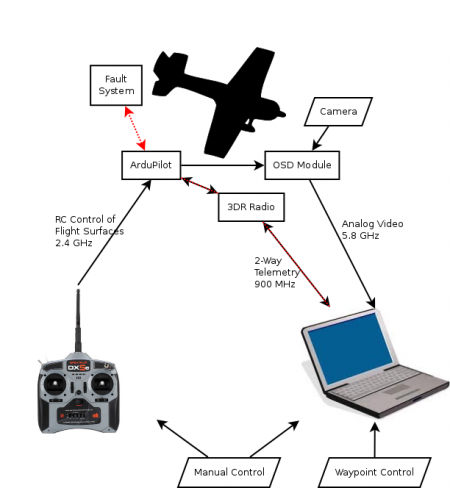
\includegraphics[scale=0.9]{figures/base_station_architecture_ardupilot.png}
\caption{Communication pipeline from Mobile device to UAV}
\label{base_station_architecture_ardupilot}
\end{figure}


\section{Interfaces and functionality: Communication between OpenCV and ROS}

Most of the artificial vision is given by the sensors of the models that we define. In order to manipulate the information we obtain through the sensors, ROS has a set of OpenCV libraries that provide the necessary tools to transform the images that are captured through the optical focus of the drone camera. In addition, it includes a large number of algorithms for odometry visual, augmented reality, machine learning and detection and recognition of objects that facilitate the use of drone controllers.

The images that are captured through the video stream of the camera are given by the topic that defines the sensor of the camera of the drone. These images are sent in a ROS sensor\_msgs/Image format. In order to manipulate these images in OpenCV it is necessary to convert them into a cv::Mat format, since it is the only compatible one. For this, there is a ROS library called cv\_bridge, which allows the transformation of ROS image to OpenCV image or otherwise OpenCV image to ROS image.


\begin{figure}[h!]
\centering
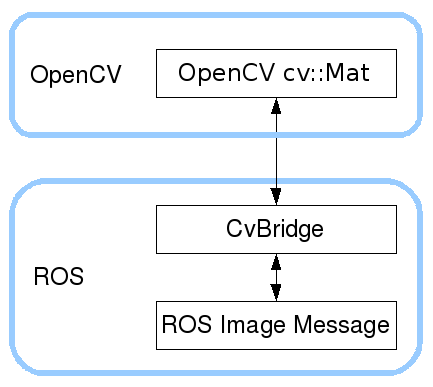
\includegraphics[scale=0.6]{figures/cv_bridge.png}
\caption{Pipeline from a ROS image to an OpenCV image}
\end{figure}

The conversion process (Algorithm 2.1) begins at the moment when our program captures the images produced by the topic that obtains the data of the camera and they begin to receive in sensor\_msgs::ImageConstPtr format. Then the transformation is done from the toCvCopy method that receives as a parameter the ROS message and the type of encoding that in this case is BGR8. As a result we obtain a structure which can be accessed in the Mat format image with CvImagePtr to image.


\section{Programming Language}

The host programming language for the Dronekit SDK as well as TensorFlow and thereby, the language that we will use to build the different functionalities of the proposed application is Python.  Python is a general purpose programming language created in the late 1980s, it is used by thousands of people to do things from testing microchips at Intel, to powering Instagram, to building video games. Python is small, very closely resembles the English language, and has hundreds of existing third-party libraries especially in computer vision hence our choice to use it since it will make our tasks simpler to perform.

\begin{figure}[h]
\centering
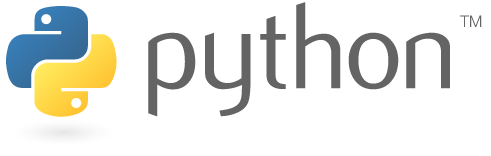
\includegraphics[scale=0.6]{figures/python.png}
\caption{Python Logo}
\end{figure}

